%!TEX root = ThesisLKN.tex
\chapter{Results and Discussions} \label{chapter:5}


\section{Metrics}

\subsection{Metrics for Neural Network}

\subsection{Metrics for Tracking}

\section{Training of Neural Network}

After the data is collected as described in Section \ref{sec:traj_sim}, we split them into training, validation and test set. The training and validation set are sampled from seven full maps, and test set is sampled from a separate map. The number of samples we generated are summarized in Table \ref{table:nos}. 

Figure \ref{fig:trajs} shows one example of map window as network input and its ground truth. On the left, a cell is labeled with red color, and the sampled trajectories that go through this cell are displayed. On the right, it shows a visualization of the ground truth \( P_c(V^{ex} | V^{en}) \) for that red cell. The axes show velocities on \( x, y\) directions. Since we assume a person has maximum speed of 1 $cell/timestep$, the velocities must be in range $[-1,1]. $Outer axes represent entering direction \( V^{en} \), and inner represents exit velocity \( V^{ex} \). One can see that \( P(V^{ex}=DL | V^{en}=DL) = 0.13 \) and \( P(V^{ex}=D | V^{en}=DL) = 0.87 \) \footnote{DL represents going down-left, and its corresponding velocity is (-1, -1). D represents going down, and its velocity is (0, -1).}. This indicates that if a person reaches the red cell by taking direction down-left (i.e., coming from upper-right neighboring cell), it is very likely that he or she will change to going down for the next time step. This proves that our way of modeling motion pattern captures human motion dynamics.

\begin{table}[t]
\centering
  \begin{tabular}{c|ccc}
    \hline
     & training & validation & test \\ \hline
    number of samples & 27,119 & 4,785 & 3,760\\
    \hline
  \end{tabular}
\caption{Number of samples in training, validation and test set.}
\label{table:nos}
\end{table}

\begin{figure}[H]
\begin{tabular}{ll}
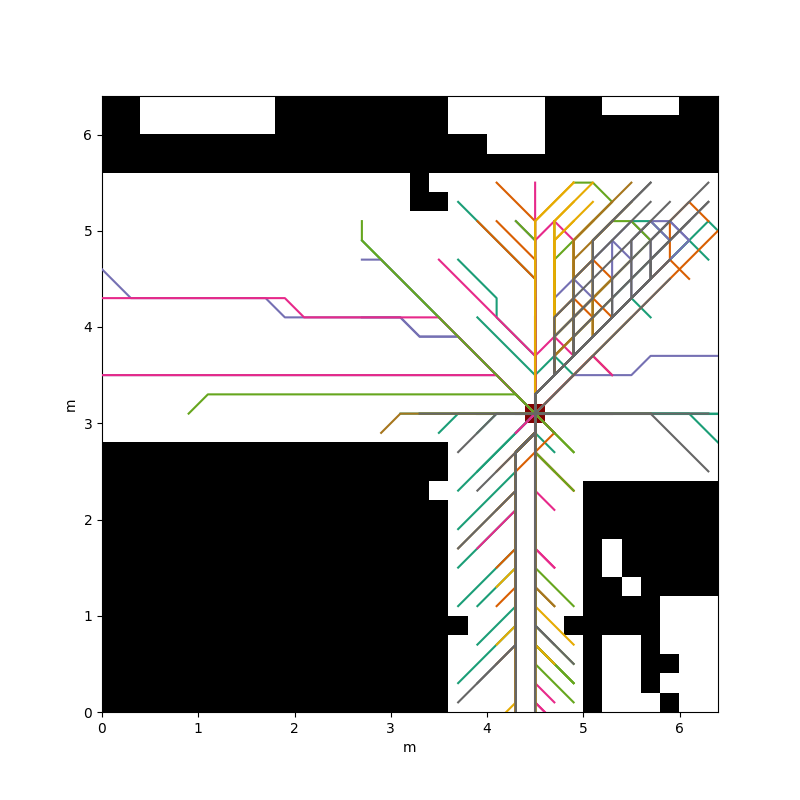
\includegraphics[width=0.48\textwidth]{figures/trajs_through_cell.png}
&
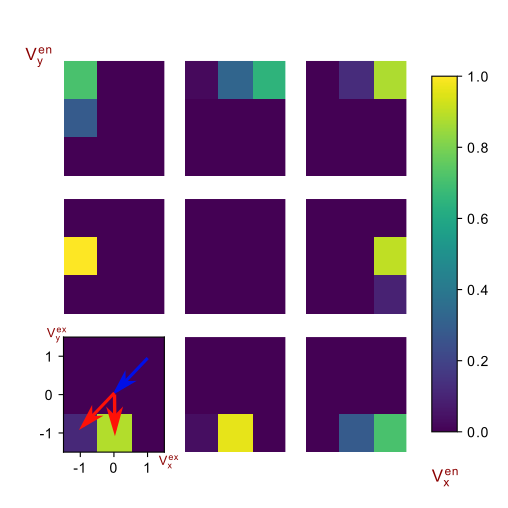
\includegraphics[width=0.48\textwidth]{figures/probs_on_that_cell_2.png}
\end{tabular}
\caption[one example of map window as network input and its ground truth]{one example of map window as network input and its ground truth \textbf{Left}: The map window has size of \( 32 \times 32 \) cells, with resolution of \( 0.2m/cell\). It also shows trajectories that goes through the red cell. \textbf{Right}: Visualization of conditional probability \( P_c(V^{ex} | V^{en}) \) for the red cell on left map. It can be seen that if a person reaches that cell by taking down-left direction, it is very like that he or she will change direction to going down.}. 
\label{fig:trajs}
\end{figure}

\section{Evaluation of Tracking Performance}

\subsection{Overview of Datasets}

\textbf{Simulated Dataset}

\textbf{Real Dataset}

\subsection{Tracking on Simulated Data}

\subsection{Tracking on Real Data}

\section{Applications}

\textbf{Dynamic Analysis}

\textbf{Get occupancy map}


 